\documentclass{article}

\usepackage{algorithm}
\usepackage[noend]{algpseudocode}

\RequirePackage{amssymb, mathptm}
\usepackage{amsbsy}
\usepackage{amsthm}
\usepackage{graphicx}
\usepackage{helvet}
\usepackage{enumerate}
\usepackage{amsmath}
\usepackage{amsfonts}
\usepackage{graphicx}
\usepackage{multirow}
\usepackage{subfig}
\usepackage{comment}
\usepackage{cases}
\usepackage{xcolor}
\usepackage{epstopdf}
\usepackage[normalem]{ulem}
\usepackage{diagbox}
\usepackage{bm}
\usepackage{hhline}

\begin{document}

\begin{algorithm}
\caption{Algorithm for performing $f+g\pmod 2$}
\label{mod2sum}
\begin{algorithmic}[1]
{\small
\Procedure{$mod\_2\_sum$}{$f,g$}
\If{$f=0$}
\State \Return $g$
\ElsIf{$g=0$}
\State \Return $f$
\ElsIf{$f=g$}
\State \Return 0
\Else
\State $v_1 = top\_var(f); v_2 = top\_var(g);$
\If{$index(v_1) < index(v_2)$}
\State \Return $ite(v_1,then(f),else(f)+g)$
\ElsIf{$index(v_1) > index(v_2)$}
\State \Return $ite(v_2,then(g),else(g)+f)$
\Else
\State \Return $ite(v_1,then(f) + then(g),else(f)+else(g))$
\EndIf


\EndIf
\EndProcedure
}
\end{algorithmic}
\end{algorithm}


{\bf ZBDD Representation:} %% We show how reduction is performed using
%% ZBDDs. 
% \subsection{ZBDD Representation}
The following steps describe the procedure for building ZBDDs for the polynomials of the gates of circuits.
\begin{enumerate}
	\item Obtain the RTTO for the variables (signals) of the circuits as $x_1 > x_2 > \dots > x_n$.
	
	\item Impose the same order on the ZBDDs. When declaring the variables, a unique index is associated with
	each variable. The index number starts from 0 and increases as we go towards the last variable in the order.
	
	\item Declare ZBDDs for each of these variables. Each of these ZBDDs contains only the root node which the variable itself,
	and the two terminal nodes with the 1-edge (0-edge) of root going into 1-terminal (0-terminal). The child 
	node of the root at the solid edge's end will be referred to as $then$ and the other child as $else$.
	
	\item Use Eqn. (\ref{b2poly}) to model the gates of the circuit as Boolean polynomials. Build ZBDDs for
	these polynomials using the $+$ and $\cdot$ binary operations for modulo 2 sum and product of variables. 
	The  $f+g\pmod 2$ operation can be implemented as $f+g = f_s \cup g_s - f_s \cap g_s$, 
	where $f_s$ and $g_s$ represent the unate cube sets for the polynomials $f$ and $g$ respectively. 
	For example, let $f = ab + c$ and $g = c + d$ with the corresponding unate cube sets
	 $f_s = \{ab,c\}$ and $g_s = \{c,d\}$, then $f_s \cup g_s = \{ab,c,d\}$ and 
	$f_s \cap g_s = \{c\}$. The set difference $f_s \cup g_s - f_s \cap g_s$ is the set $\{ab,d\}$
	and the corresponding Boolean polynomial is $ab + d$. 
	\par	However, analysis from experiments shows that the union $f_s \cup g_s$ can introduce a
	large number of terms (large ZBDD size) which are eventually canceled when performing the set difference.
	In order to avoid the large ZBDD size for the union operation we have implemented the $f+g\pmod 2$
	operation as presented in~\cite{polybori:2009}. The algorithm for this operation is shown in
	Algorithm \ref{mod2sum}. 
	\par In the above algorithm, the function $top\_var$ returns the root variable
	for the input ZBDD ($f$ or $g$). The function $ite$ is an $if$-$then$-$else$
	operator used for constructing new ZBDDs. The algorithm first checks the  
	simple corner cases in the beginning of the algorithm and then depending
	on the index values of the variables (which in our case is RTTO) it recursively constructs 
	new ZBDDs using the $ite$ function. 

	\par In the above example, let the ordering imposed on the variables is $a>b>c>d$ and the 
	index values for these variables are $0,1,2,3$ respectively. For the given $f$ and $g$ $i.e.$
	$ab+c$ and $c + d$ respectively, the condition $index(v_1) < index(v_2)$ is true. The $ite$ operation places
	$then(f) = b$ on the solid edge of the root of the new ZBDD and performs $else(f) + g \pmod2$ for the 
	dotted edge's end as shown in the Fig. \ref{mod2sumfig}. During this recursive call, the last condition is true 
	(as $index(v_1) = index(v_2) = 2$). This time the  $ite$ operation performs two recursive calls $then(f) + then(g)$ and 
	$else(f) + else(g)$. The recursive call $then(f) + then(g)$ returns 0 as 
	both of them are 1 whereas the recursive call $else(f) + else(g)$ returns $d$ as $else(f) = 0$
	and $else(g) = d$. Therefore $ite$ operation creates a ZBDD with root $c~(= v_1 = v_2)$ and its 1-$child$
	pointing to 0 and 0-$child$ pointing to $d$. Due to the ZBDDs' reduction rules, it gets simplified to 
	just $d$. Therefore, the resultant ZBDD of the operation $(ab+c)+(c+d)$ has $a$ as its root,
	1-$child$ as $b$, and 0-$child$ as $d$ while representing the boolean polynomial $ab+d$.
 
	A similar recursive algorithm is also implemented for $f\cdot g \pmod 2$ operation
	where the intermediate partial product terms are added using the Algorithm \ref{mod2sum}.

	\item Traversing only the solid edges from the root node of a ZBDD to
    terminal {\bf 1} delivers the leading monomial of that polynomial.  
  
\end{enumerate} 

\begin{figure}[hbt]
\centering
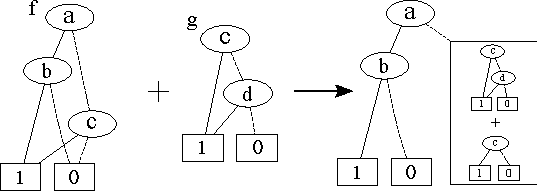
\includegraphics[scale=1]{mod2sumfig.pdf}
\caption{$f+g\pmod 2$ using ZBDDs}
\label{mod2sumfig}
\end{figure}

\end{document}
